% =====================================================================
% EMMET paper v2 - master document.
% Assembles the v2 sections around the elegance/equivalence thesis.
% Compile: pdflatex paper_v2.tex (twice for refs)
% =====================================================================
\documentclass[11pt]{article}
\usepackage[T1]{fontenc}
\usepackage[utf8]{inputenc}
\usepackage[a4paper,margin=2cm]{geometry}
\usepackage[ruled,vlined]{algorithm2e}
\usepackage{amsmath, amssymb}
\usepackage{graphicx}
\usepackage{cite}
\usepackage{booktabs}
\usepackage{xcolor}
\usepackage{hyperref}
\hypersetup{colorlinks=true, linkcolor=blue!50!black, citecolor=blue!50!black}

\title{When Topology Decides the Load:\\
\large A Structural Attractor in Graph Routing,\\
Found Through Classical-Physics Heuristics}
\author{Carlos L\'opez}
\date{Draft v3 --- \today}

\begin{document}
\maketitle

% Abstract v4 - attractor-first thesis. Physics as discovery tool, not claim.
% Honest about margin-sensitivity; structural attractor as the headline.
\begin{abstract}
Load balancing on a graph is usually framed as an algorithm-design problem: a
better router yields a better load distribution. We report evidence that, over
a wide range of topologies, the load distribution is instead largely fixed by
the structure of the graph and the traffic demand, leaving any reasonable
congestion-aware router little freedom---and we identify a topological metric
that predicts how much freedom remains. We reached this through an unusual
route. Treating a packet as a particle under a classical force, we built three
independent routing cores---a Newtonian loss-reaction, an Archimedean buoyancy,
and a Pascalian pressure diffusion---sharing a search engine but no mechanism.
The three produce near-identical per-edge load distributions (cosine $0.99$),
significantly tighter than blind controls such as ECMP ($0.87$), and reach
statistical equivalence (TOST) with the engineered balancers CONGA and DRILL on
most of fifteen topologies. A sensitivity analysis is candid about the limits of
that equivalence: at a strict margin ($0.5$ percentage points of drop rate) only
a few topologies remain equivalent, and they are precisely the ones where the
structural attractor is strongest. We argue, via a cut-based structural
argument, that this is no coincidence: the demand fixes the flow across every
cut, the topology's cut structure pins most of the load distribution, and any
congestion-aware rule---physical or engineered---shapes the small residual
identically. A purely structural ratio, tube/sp (room to manoeuvre among
near-shortest paths, computable before deployment), predicts where the residual
is large enough for routers to differ; the correlation is robust to leave-one-out
and strengthens when the loosest-fitting topologies are removed ($r$ rising from
$0.78$ to $0.89$). The physics, in the end, was a discovery instrument rather
than the result: three classical analogies converged because the problem, not
the analogy, drove them to the same place. We report our negative results, an
audit retracting an earlier inflated advantage, and the margin sensitivity in
full.
\end{abstract}


% ====================================================================
% Section 1 (v2): Introduction.
% Written last, with the whole body in place. Voice: physics-first,
% honesty as a feature, equivalence-not-dominance.
% ====================================================================
\section{Introduction}
\label{sec:intro}

Network load balancing is a mature engineering discipline. Production systems
such as CONGA~\cite{conga} and DRILL~\cite{drill} spread traffic across a
network using carefully designed mechanisms: per-flowlet rerouting, multi-path
candidate enumeration, local queue sampling, and centrally or distributively
maintained congestion state. These systems work well, and improving on them is
hard.

This paper does not try to improve on them. It asks a different and, we think,
more interesting question:

\begin{quote}
\emph{How much of what engineered load balancers achieve can be recovered from
classical physics alone---from a packet treated as a particle obeying a couple
of elementary mechanical laws?}
\end{quote}

The motivation is partly methodological. An expert in routing reasons within
the conceptual vocabulary of routing; a physicist handed the same problem
reasons about gradients, forces, and conservation laws. Occasionally the second
framing reaches a familiar destination by an unfamiliar and more economical
road, and the comparison is informative regardless of which arrives first. Our
interest is therefore not a horse race but a question of \emph{parsimony}: how
little mechanism suffices to reach the operating point that elaborate
engineering reaches.

\subsection{The model, in one paragraph}

We treat a packet as a particle descending a potential field defined on the
network graph. The particle feels two forces. The first is a \emph{gradient}:
it rolls toward lower latency and lower congestion, subject to a hop budget that
lets it take a modestly longer, emptier detour rather than forcing every packet
onto the single shortest path. The second is a \emph{reaction} in the sense of
Newton's third law: when a packet is dropped on a congested edge, it pushes
back, depositing a decaying ``scar'' that steers subsequent packets away from
edges that have just failed. That is the entire router---two terms, no central
controller, no per-flow state, no precomputed path tables, sixty lines of code.

\subsection{What we find}

Our central result is deliberately stated as an \emph{equivalence}, not a
victory:

\begin{enumerate}
\item \textbf{Two terms suffice.} The two-term core is the survivor of an
ablation: an earlier model carried eight physically-motivated layers (effective
mass, a thermostat, a temporal ripple, buoyancy), and measurement showed that
only the gradient and the Newton-III scar earn their keep---the rest are inert
or mildly harmful (Section~\ref{sec:ablation}).

\item \textbf{It matches engineered routers.} Tested as a statistical
equivalence (TOST, margin $2$ percentage points) across fifteen topologies in a
flow-level simulator, the core is equivalent to DRILL on twelve of fifteen, and
equivalent to CONGA once CONGA is given a fair path budget. It reaches the same
operating point CONGA reaches only after enumerating and scoring sixteen to
thirty-two candidate paths per flow (Sections~\ref{sec:equivalence}--\ref{sec:fair}).

\item \textbf{A topological metric predicts when.} A quantity computable from
the graph alone, the tube/sp ratio (room to manoeuvre among near-shortest
paths), predicts where the equivalence holds and where engineered multi-path
routing keeps a genuine edge (Pearson $r = 0.78$); the two real WAN backbones,
with low tube/sp, are exactly the predicted exceptions
(Section~\ref{sec:applicability}).
\end{enumerate}

The upshot is that two classical forces, with none of the apparatus of modern
load balancers, reach the same place those balancers reach, on the topologies
where the geometry leaves room to do so---and that the qualifying clause is
itself predictable.

\subsection{A note on method}

This paper reports its negative results and its own corrections in full.
The eight-layer model is presented and then dismantled; an early, larger
advantage over CONGA is shown to have been an artifact of an unfair path budget
and is retracted (Section~\ref{sec:fair}). We regard this not as throat-clearing
but as the substance of the contribution: a claim that physics matches
engineering is worth precisely as much as the adversarial scrutiny it has
survived, and we would rather report an honest equivalence than an inflated
win. Every headline figure here has been checked against the strongest version
of its baseline we could build.


% ====================================================================
% Section 2 (v2): Related work.
% Positions the contribution as parsimony, not SOTA competition.
% ====================================================================
\section{Related Work}
\label{sec:related}

\paragraph{Engineered load balancing.}
Modern multipath load balancers spread traffic to avoid hot spots.
ECMP~\cite{ecmp} splits flows across equal-cost shortest paths by hashing, with
no congestion awareness. CONGA~\cite{conga} adds that awareness: it enumerates a
set of candidate paths and selects among them using in-network congestion
feedback, rerouting at flowlet granularity. DRILL~\cite{drill} pushes the
decision to the switch and the microsecond, making per-packet local choices
based on queue occupancy with minimal state. These systems define the operating
points we measure against. Our aim is not to outperform them---on the
topologies where they are strong, they remain strong---but to ask how much of
their behaviour is recoverable from a far simpler, physically-motivated rule.

\paragraph{Physics- and nature-inspired routing.}
Using physical or biological analogies for routing has a long history:
ant-colony optimisation, electrical-network and resistance analogies,
potential- and field-based forwarding, and physarum-inspired path formation.
These approaches typically introduce a mechanism and demonstrate that it works.
Our contribution differs in emphasis in two ways. First, we run the analogy in
reverse as an ablation: rather than showing that added physics helps, we add a
great deal of physics and then measure how much can be removed, arriving at a
two-term residue. Second, we frame the outcome as a statistical equivalence
against strong engineered baselines, rather than as a demonstration that the
physical method is novel or superior.

\paragraph{Equivalence testing.}
Most networking evaluations test for a difference (one method beats another).
We instead test for \emph{equivalence}, using TOST (two one-sided
tests), which asks whether two methods are indistinguishable within a stated
margin. This is the statistically appropriate tool when the claim is ``as good
as'', not ``better than'', and it guards against the familiar error of reading a
non-significant difference as evidence of equivalence. To our knowledge,
equivalence testing is uncommon in the routing-evaluation literature, and its
use here is deliberate: the entire thesis is one of equivalence with parsimony.

\paragraph{Applicability conditions.}
A recurring weakness of method papers is silence about when the method fails. We
attach to our result an explicit, topology-only predictor (the tube/sp ratio,
Section~\ref{sec:applicability}) that says in advance where the equivalence
holds and where engineered routing retains an edge. This places the
contribution closer to the spirit of complex-systems and network-science work,
where structural predictors of dynamical behaviour are themselves the object of
study, than to a conventional systems-performance paper.


\medskip
Conceptually adjacent, though router-free, is the literature on dynamic
averaging and load-balancing processes on graphs, e.g.\ Alistarh et
al.~\cite{alistarh2022dynamic}, where iterative local exchanges converge
to equilibria fixed by graph structure. The attractor reported in this
paper is the routing-level analogue of that structural determinism,
observed empirically across heterogeneous mechanisms rather than proved
for a single dynamics.


% ====================================================================
% Section 3 (v2): The two-term physical core.
% Replaces the 8-layer "mass-aware" model of v1. Faithful to
% experiments/emmet_core.py.
% ====================================================================
\section{The Two-Term Physical Core}
\label{sec:core}

\noindent\emph{(Presented as built: Section~\ref{sec:redux} re-audits this core on the modern bench and inverts which term earns its place.)}

We model a packet as a classical particle descending a potential field
defined on the network graph. The particle is subject to two forces, and
only two. We state them first, then justify by ablation
(Section~\ref{sec:ablation}) that no further mechanism is needed.

\subsection{The potential}

Each directed traversal of an edge $(u,v)$ carries a cost
\begin{equation}
\phi(u,v) \;=\; \alpha\,\ell(u,v) \;+\; \beta\,\frac{x(u,v)}{c(u,v)} \;+\; \gamma\,s(u,v),
\label{eq:potential}
\end{equation}
where $\ell$ is edge latency, $x/c$ is the instantaneous load-to-capacity
ratio (congestion), and $s$ is a persistent \emph{scar} term defined below.
The three weights $(\alpha,\beta,\gamma)$ are the only tunable quantities of
the model. All three are local: computing $\phi$ needs no global state beyond
the edge itself.

\subsection{Force 1: gradient descent}

The particle follows the downhill direction of $\phi$ from source to
destination, subject to a hop budget: it may use a path no longer than
$\lceil \alpha_{\text{budget}}\, h_{\text{sp}} \rceil$ hops, where
$h_{\text{sp}}$ is the shortest-path hop count. The minimum-potential path
under this budget is found exactly by a dynamic program over
$(\text{hops used},\, \text{node})$, in $O(k\,|E|)$ time with
$k=\lceil\alpha_{\text{budget}} h_{\text{sp}}\rceil$.
The budget is what lets the particle take a slightly longer, less congested
detour instead of forcing every packet onto the single shortest path---the
mechanism by which load spreads.

% Algorithm 1: the two-term core routing step. Uses algorithm2e.
\begin{algorithm}[t]
\caption{EMMET-core routing step (two-term physical router)}
\label{alg:core}
\SetAlgoLined
\KwIn{graph $G=(V,E)$ with per-edge latency $\ell$, load $x$, capacity $c$;
scar field $s$; source $a$, destination $z$; weights $\alpha,\beta,\gamma$;
budget factor $\alpha_b$}
\KwOut{path $a \rightsquigarrow z$}
$h_{\text{sp}} \leftarrow$ shortest-path hop count $a \to z$\;
$k \leftarrow \lceil \alpha_b \, h_{\text{sp}} \rceil$\tcp*{hop budget}
\For{each edge $(u,v)$}{
  $\phi(u,v) \leftarrow \alpha\,\ell(u,v) + \beta\,x(u,v)/c(u,v) + \gamma\,s(u,v)$\;
}
$P \leftarrow$ min-$\sum\phi$ path of length $\le k$ via DP over (hops, node)\tcp*{$O(k|E|)$}
\Return $P$\;
\BlankLine
\tcp{On a drop at edge $(u,v)$ while forwarding:}
$s(u,v) \leftarrow s(u,v) + 1$\tcp*{Newton-III reaction}
\tcp{Once per step, everywhere:}
$s \leftarrow \rho\, s$, \quad $\rho = 2^{-1/T_{1/2}}$\tcp*{scars fade}
\end{algorithm}


\subsection{Force 2: Newton's third law (the scar)}

The gradient term reacts to congestion that is \emph{present}. It cannot
react to congestion that has just \emph{caused a loss}: once a packet is
dropped, the offending edge's instantaneous load may already have fallen.
We close this gap with a reaction term inspired by Newton's third law---to
every action a packet undergoes, the network responds with an equal and
opposite reaction on the packets that follow.

Concretely, when a packet is dropped on edge $(u,v)$, that edge's scar is
incremented, $s(u,v) \leftarrow s(u,v) + 1$. The scar enters the
potential~\eqref{eq:potential} with weight $\gamma$, so subsequent particles
feel a repulsive reaction steering them away from edges that recently
failed---information the instantaneous congestion term does not carry.

Scars are not permanent: at each step they decay,
$s(u,v) \leftarrow \rho\, s(u,v)$ with $\rho = 2^{-1/T_{1/2}}$ and half-life
$T_{1/2}$. A corridor that stops failing reopens on its own, and at rest
(no losses) the scar field vanishes and the router reduces to pure gradient
descent. The mechanism is self-regulating: it acts only when and where the
network is actually breaking. This is the only memory in the model, and---as
the ablation will show---the only added mechanism that earns its keep.

\subsection{What is deliberately absent}
\label{sec:absent}

This two-term core is the survivor of a larger model. Earlier versions of
EMMET endowed the packet-particle with extra physical attributes: an
effective mass that grew with traversed congestion, a network thermostat
modulating the congestion weight, a temporal ripple diffusing loss memory
over several steps, and an Archimedes-style buoyancy term. Each was
physically motivated and individually plausible.

A systematic ablation (Section~\ref{sec:ablation}) removed them one at a time
and measured the cost. The result was unambiguous: the gradient and the
Newton-III scar account for essentially all of the performance, while the
remaining mechanisms ranged from negligible to mildly harmful---removing the
ripple and the thermostat slightly \emph{improved} results. We therefore
report the two-term core as the model and treat the richer apparatus as a
cautionary tale about physically-seductive terms that do not survive
measurement. The reference implementation is 60 lines of Python.



% ====================================================================
% Section 4 (v2): The ablation - why two terms and not eight.
% Faithful to data/ablation_raw.json (cap 2,2) and ablation_24_raw.json (cap 2,4).
% Numbers are the change in losses when each layer is REMOVED from the full model.
% ====================================================================
\section{Ablation: Why Two Terms}
\label{sec:ablation}

Section~\ref{sec:core} asserted that only two mechanisms survive scrutiny. This
section is the evidence. EMMET did not begin parsimonious; it began as an
exercise in taking the particle metaphor seriously, and accreted eight physical
layers. We removed them one at a time and measured what each was worth.

\subsection{The candidate layers}

Beyond the gradient (which is the irreducible substrate---without it there is no
router) the full model carried four added mechanisms:

\begin{itemize}
\item \textbf{Newton-III scar} (loss-reaction memory, Section~\ref{sec:core}).
\item \textbf{Effective mass}: a packet's influence on the potential grew with
the congestion it had already traversed, modelling inertia.
\item \textbf{Thermostat}: a global network ``temperature'' that scaled the
congestion weight $\beta$ as mean utilisation rose.
\item \textbf{Temporal ripple}: loss memory deposited not as a single
increment but diffused over several subsequent steps, like a wave.
\end{itemize}

\subsection{Protocol}

We evaluated the full model and four leave-one-out variants (each removing a
single layer), plus a bare core (gradient only, all four layers removed),
against the trivial-but-stateless DRILL baseline on the G\'EANT backbone under
trunk-link failure. Two load regimes were used---moderate (capacity drawn from
$[2,4]$) and saturated ($[2,2]$)---across the failed-link ensemble with 30
seeds each. The quantity of interest is the \emph{change in total losses when a
layer is removed} from the full model: a positive change means the layer was
doing useful work; a negative or zero change means it was inert or harmful.

\subsection{Result: only the scar earns its keep}

Table~\ref{tab:ablation} reports the change in losses on removal of each layer,
in both regimes.

\begin{table}[t]
\centering
\caption{Change in total losses when each layer is removed from the full model
(positive = the layer was helping; negative = it was hurting). G\'EANT, trunk
failure, 30 seeds. The Newton-III scar is the only layer whose removal clearly
hurts; the ripple's removal slightly \emph{helps}.}
\label{tab:ablation}
\small
\begin{tabular}{lcc}
\toprule
Layer removed & moderate load & saturated load \\
\midrule
Temporal ripple   & $-0.4\%$ & $-0.5\%$ \\
Thermostat        & $\phantom{+}0.0\%$ & $\phantom{+}0.0\%$ \\
Effective mass    & $+4.2\%$ & $+1.6\%$ \\
Newton-III scar   & $+16.7\%$ & $+6.4\%$ \\
\midrule
All four (bare core) & $+38.7\%$ & $+9.8\%$ \\
\bottomrule
\end{tabular}
\end{table}

The reading is blunt:

\begin{itemize}
\item The \textbf{Newton-III scar} is the one added layer that earns its keep:
removing it raises losses by $6.4$--$16.7\%$. It is doing the real work.
\item \textbf{Effective mass} contributes marginally ($1.6$--$4.2\%$).
\item The \textbf{thermostat} has \emph{no measurable effect} (0.0\% in both
regimes): it is pure decoration.
\item The \textbf{temporal ripple} is mildly \emph{harmful}: removing it
slightly improves results. The most physically evocative layer---a wave of loss
memory rippling outward---was a net negative.
\end{itemize}

Removing all four at once (the bare gradient core) costs $9.8$--$38.7\%$,
confirming that the gradient alone is not enough: it needs the scar. But it
needs \emph{only} the scar. The mass, thermostat, and ripple together account
for almost nothing, and the ripple actively hurts.

\subsection{Interpretation}

This is the parsimony result that gives the paper its title. Of the eight-layer
apparatus, the data retain exactly two mechanisms---gradient descent and the
Newton-III scar---and discard the rest. Crucially, the discarded layers were not
obviously bad ideas: effective mass, thermal scaling, and wave-like diffusion
are all physically natural, and each had a plausible story. They simply did not
survive measurement. We take this as a methodological lesson worth stating
explicitly: in physics-inspired modelling, the seductiveness of a mechanism is
no evidence of its usefulness, and only ablation tells them apart. The two-term
core of Section~\ref{sec:core} is what remained standing.


% ====================================================================
% Section 5 (v2): The equivalence experiment.
% The heart of the reframed paper. Faithful to experiments/equivalence.py
% and data/equivalence_results.txt + data/fair_comparison_results.txt.
% ====================================================================
\section{Equivalence with Engineered Routers}
\label{sec:equivalence}

The central claim of this paper is deliberately modest and precisely
testable:

\begin{quote}
\emph{The two-term physical core reaches the operating point of
purpose-built load balancers across most topologies, using a fraction of
their machinery; and a topological metric predicts the cases where it does
not.}
\end{quote}

We test this as a statistical \emph{equivalence} claim, not a superiority
claim. The distinction matters: showing that two methods are
indistinguishable requires a different test than showing one beats the
other, and conflating the two is a common error.

\subsection{Design}
\label{sec:equiv-design}

We compare the two-term core (gradient + Newton-III, no mass) against two
engineered baselines: \textbf{CONGA}, a multi-path congestion-aware balancer
that scores $K$ shortest paths and selects the least congested, and
\textbf{DRILL}, a near-stateless balancer that makes per-hop local decisions.
ECMP and shortest-path serve as weak controls the physical core is expected
to beat.

All routers are evaluated in a flow-level simulator: a flow is born, lives
for several ticks injecting sustained load along its route, then dies. This
matters because routing behaviour differs between the packet-bullet regime
(where DRILL's per-hop reactivity shines) and the flow regime (where choosing
a whole path well at birth matters more). We report the flow regime as the
more realistic of the two for backbone traffic.

We sweep \textbf{15 topologies} spanning four families: regular lattices
(grids $5\times5$ to $12\times12$), small-world (Watts--Strogatz, several
sizes and degrees), scale-free (Barab\'asi--Albert), and two real WAN
backbones (G\'EANT, Abilene). Each topology is run with $n=20$ seeds. The
performance metric is the drop rate (fraction of flow-ticks that hit an
overloaded edge; lower is better).

\subsection{Equivalence test}

For each topology we test equivalence between the core and each baseline with
\textbf{TOST} (two one-sided tests) on the paired per-seed drop rates, with an
equivalence margin $\delta = 2$ percentage points. TOST declares equivalence
only when the $90\%$ confidence interval of the mean difference lies entirely
within $[-\delta, +\delta]$: that is, when we can reject \emph{both} the
hypothesis that the core is worse by more than $\delta$ \emph{and} that it is
better by more than $\delta$. This is a stricter, more honest bar than
observing overlapping confidence intervals.

\subsection{Results}
\label{sec:equiv-results}

Table~\ref{tab:equivalence} reports the per-topology drop rates and TOST
verdicts. The core is statistically equivalent to DRILL on
\textbf{12 of 15 topologies}. Against CONGA at its default budget ($K=4$) the
formal equivalence count is lower (5 of 15), but---crucially---most of the
non-equivalences are cases where the core is \emph{better}, not worse: on the
larger grids the core's drop rate is $0.002$--$0.005$ versus CONGA's
$0.034$--$0.066$. We examine this apparent advantage critically in
Section~\ref{sec:fair}, where it turns out to be an artifact of CONGA's path
budget rather than a genuine physical superiority.

\begin{table}[t]
\centering
\caption{Drop rate (lower is better) of the two-term core versus engineered
baselines across 15 topologies, flow regime, $n=20$ seeds. ``$\equiv$D'' and
``$\equiv$C'' mark TOST equivalence ($\delta=2$pp) with DRILL and CONGA$_{K=4}$
respectively.}
\label{tab:equivalence}
\small
\begin{tabular}{lccccc}
\toprule
Topology & core & CONGA$_{K=4}$ & DRILL & $\equiv$D & $\equiv$C \\
\midrule
Grid $5$      & 0.018 & 0.029 & 0.032 &     &     \\
Grid $6$      & 0.011 & 0.024 & 0.023 & yes & yes \\
Grid $7$      & 0.011 & 0.027 & 0.022 & yes &     \\
Grid $8$      & 0.005 & 0.034 & 0.015 & yes &     \\
Grid $10$     & 0.003 & 0.050 & 0.019 &     &     \\
Grid $12$     & 0.002 & 0.066 & 0.009 & yes &     \\
WS $n30\,k4$  & 0.016 & 0.033 & 0.004 & yes &     \\
WS $n50\,k4$  & 0.023 & 0.040 & 0.009 &     &     \\
WS $n50\,k6$  & 0.005 & 0.007 & 0.000 & yes & yes \\
WS $n80\,k4$  & 0.022 & 0.037 & 0.008 & yes &     \\
BA $n50\,m2$  & 0.003 & 0.001 & 0.000 & yes & yes \\
BA $n50\,m3$  & 0.000 & 0.000 & 0.000 & yes & yes \\
BA $n80\,m2$  & 0.001 & 0.001 & 0.000 & yes & yes \\
G\'EANT       & 0.057 & 0.042 & 0.053 & yes &     \\
Abilene       & 0.057 & 0.042 & 0.053 & yes &     \\
\bottomrule
\end{tabular}
\end{table}

The scale-free topologies (Barab\'asi--Albert) sit near zero drop for every
router: their hub structure leaves little congestion to redistribute, so
equivalence there is trivial and we do not lean on it. The informative cases
are the grids, the small-world graphs, and the real backbones.

\subsection{Limitations of this experiment}

Two caveats are stated plainly, and the first records a correction. An audit
of the harness behind this bench found that its `Abilene' entry had been
loading the G\'EANT graph under a second name: every Abilene figure that
harness produced---including the Abilene row of
Table~\ref{tab:equivalence}---was G\'EANT counted twice. The harness is fixed
in this revision: Abilene is now the real eleven-node backbone with its own
independent demand, restoring a bench of fifteen genuine topologies, and all
results from Section~\ref{sec:margin-sensitivity} onward use it. The corrected
Abilene turns out to be the bench's saturation regime (drop rates above
$20\%$), where no physical core reaches equivalence at any margin
(Sections~\ref{sec:margin-sensitivity} and~\ref{sec:twofactor});
Table~\ref{tab:equivalence} retains the historical row within the $K{=}4$
presentation that Section~\ref{sec:fair} audits, and the regenerated table at the fair
budget, on the corrected bench, is Table~\ref{tab:fairbench}
(Section~\ref{sec:fairbench}).
Second, the equivalence margin $\delta=2$pp is an \emph{operational} threshold, not an arbitrary one: two percentage points of sustained drop rate is the scale at which a capacity planner would treat two schemes as materially different, while smaller gaps are absorbed by the provisioning headroom production backbones already carry (Section~\ref{sec:margin-sensitivity} anchors this magnitude and separates operational from statistical equivalence);
Section~\ref{sec:margin-sensitivity} analyses how the verdicts behave as it
tightens, and we report raw drop rates alongside the verdicts so a reader who
prefers a different margin can reinterpret the table directly.


% ====================================================================
% Margin-sensitivity analysis of the TOST equivalence.
% Turns the reviewer critique (delta=2pp is lax) into honest evidence
% that REINFORCES the attractor reading. Goes into the equivalence section.
% Data: data/equivalence_strict_{newton,archimedes,pascal}.json
% ====================================================================
\subsection{How far does the equivalence hold? A margin-sensitivity analysis}
\label{sec:margin-sensitivity}

An equivalence verdict means nothing without stating the margin, and the choice
of $\delta = 2$ percentage points of drop rate deserves justification rather
than assertion. We anchor it operationally. A drop-rate difference is a
sustained loss differential: on a $10$\,Gbit/s backbone link under typical load,
$2$ pp of drop rate is on the order of a few hundred Mbit/s of sustained loss,
the scale at which a capacity planner provisions additional headroom or treats
two schemes as materially different. Below that scale the difference is real but
operationally inert---it disappears into the over-provisioning margin that
production backbones already carry.
The $2$ pp margin therefore marks the boundary of \emph{operational}
equivalence: differences a deployed network would act on, not the finest
difference a statistical test can resolve. We are explicit that these are
different claims. At a strict statistical margin the engineered and physical
schemes are distinguishable; what we show is that across most topologies they
are \emph{operationally} equivalent, and we now map exactly how far that holds
as $\delta$ tightens.

We therefore re-ran TOST at progressively stricter margins for all three cores. Table~%
\ref{tab:margins} reports how many of the fifteen topologies remain equivalent
to CONGA$_{K=16}$ and DRILL as $\delta$ tightens from $2.0$ to $0.2$ pp.

\begin{table}[t]
\centering
\caption{Number of topologies (of 15) at which each core is TOST-equivalent to
CONGA$_{K=16}$ / DRILL, as the equivalence margin $\delta$ tightens. The
equivalence is margin-sensitive for all three cores; what survives the strict
margins concentrates on the strong-attractor topologies.}
\label{tab:margins}
\small
\begin{tabular}{lcccc}
\toprule
core & $\delta=2.0$pp & $\delta=1.0$pp & $\delta=0.5$pp & $\delta=0.2$pp \\
\midrule
Newton     & 9 / 10  & 5 / 7 & 2 / 3 & 0 / 0 \\
Archimedes & 12 / 10 & 5 / 5 & 3 / 2 & 2 / 2 \\
Pascal     & 10 / 10 & 6 / 6 & 2 / 2 & 1 / 0 \\
\bottomrule
\end{tabular}
\end{table}

We read this honestly: the headline equivalence counts of $9$--$12$ of $15$ rest
on the $2$ pp margin, and thin out sharply under a strict one. This is the
expected behaviour, not a failure, and it sharpens rather than weakens the
paper's thesis. The equivalences that survive a strict margin are not random:
they concentrate on the scale-free (Barab\'asi--Albert) topologies, where drop
rates are near zero for \emph{every} router because the hub structure leaves
little congestion to distribute. Those are precisely the topologies where the
load-distribution attractor of Section~\ref{sec:attractor} is strongest---where
the cut structure pins almost the entire distribution and no router has room to
do better or worse. Equivalence is bulletproof exactly where the topology
removes the router's freedom, and margin-sensitive exactly where the topology
grants it. The margin analysis and the attractor are the same finding measured
two ways: \emph{the engineered/physical distinction matters only to the extent
the topology lets it}. The corrected real Abilene sharpens the point from the other side: the bench saturation regime reaches equivalence at \emph{no} margin for any core---the boundary the two-factor law of Section~\ref{sec:twofactor} requires.


% ====================================================================
% Section 6 (v2): The fair-comparison audit.
% Turns the apparent grid "win" into honest equivalence.
% Faithful to data/fair_comparison_results.txt.
% ====================================================================
\section{A Fair-Comparison Audit}
\label{sec:fair}

Section~\ref{sec:equiv-results} left a loose end: on the regular grids the
two-term core appeared to crush CONGA, with drop rates an order of magnitude
lower ($0.002$--$0.005$ versus $0.034$--$0.066$). A superiority that large,
appearing only on the most regular topologies, is exactly the kind of result
that should invite suspicion rather than celebration. We audited it, and it
did not survive.

\subsection{The suspicion}

CONGA selects among the $K$ shortest paths between a source and destination.
We had run it at its conventional default, $K=4$. On a regular lattice,
however, the $K$ shortest paths between two nodes are near-identical: they are
all minimal-length staircases differing only in the order of their horizontal
and vertical steps. With $K=4$, CONGA's four candidates are four almost
interchangeable staircases through the same congested region---it was not
being outrouted, it was being \emph{path-starved}. The physical core, which
searches all paths within its hop budget via the dynamic program, was simply
considering routes that CONGA was never offered.

If this diagnosis is correct, then widening CONGA's path budget should close
the gap on exactly these topologies, and leave the real-backbone result
(where shortest paths are genuinely diverse) largely unchanged.

\subsection{The test}

We re-ran CONGA with $K \in \{4, 16, 32\}$ on the grids, a small-world
control, and G\'EANT (Table~\ref{tab:fair}). The prediction holds cleanly.

\begin{table}[t]
\centering
\caption{Drop rate of the two-term core versus CONGA at increasing path
budgets $K$. On regular topologies a fair budget ($K=16$--$32$) closes the gap
entirely; on the real backbone the budget barely matters. Lower is better,
$n=12$.}
\label{tab:fair}
\small
\begin{tabular}{lcccc}
\toprule
Topology & core & CONGA$_{K=4}$ & CONGA$_{K=16}$ & CONGA$_{K=32}$ \\
\midrule
Grid $8$    & 0.004 & 0.034 & 0.006 & 0.002 \\
Grid $10$   & 0.004 & 0.061 & 0.011 & 0.004 \\
Grid $12$   & 0.001 & 0.066 & 0.015 & 0.005 \\
WS $n50\,k4$ & 0.024 & 0.032 & 0.012 & 0.009 \\
G\'EANT     & 0.055 & 0.040 & 0.028 & 0.034 \\
\bottomrule
\end{tabular}
\end{table}

On the grids, raising $K$ from $4$ to $32$ takes CONGA from roughly $15\times$
worse than the core to level with it or slightly ahead (Grid~$10$:
$0.061 \to 0.004$, matching the core's $0.004$). On the small-world control
the same convergence appears. On G\'EANT, where the shortest paths are already
diverse, the path budget barely moves the result---CONGA is competitive at
$K=4$ and stays so.

\subsection{What the audit means}

The grid ``win'' was an artifact of an unfair path budget, and we retract it.
This is not a setback for the paper's thesis; it sharpens it. The honest
statement is not that the physical core \emph{beats} CONGA, but that it
\emph{reaches the same operating point by a different and cheaper route}:

\begin{quote}
The two-term core attains, through a local gradient computation with no
precomputed paths, the performance that CONGA reaches only after enumerating
and scoring $16$--$32$ candidate paths per flow.
\end{quote}

Same destination, far less machinery. On a regular grid the physical rule
finds good detours for free that CONGA finds only when explicitly handed
enough candidates; on a real backbone the two are simply equivalent. In no
case does the physics need to be cleverer than the engineering---which is
precisely the claim. Equivalence with parsimony, not dominance.

\subsection{A note on auditing one's own results}

We report this audit in full, including the retracted numbers, because the
discipline it embodies is part of the contribution. A two-term physical model
that matches engineered routers is interesting only if the comparison is fair;
the value of the result is exactly as good as the adversarial scrutiny it has
survived. Every headline figure in this paper has been checked against the
strongest, best-resourced version of its baseline we could construct.


% ====================================================================
% Section: Convergence of independent classical-physics cores.
% The new centerpiece. Faithful to data/equivalence_{newton,archimedes,
% pascal}.json, all measured on the identical CONGA-K16 / DRILL / TOST bench.
% ====================================================================
\section{Convergence: Three Classical Physics, One Destination}
\label{sec:convergence}

If a single physically-motivated rule matched engineered routing, it could be a
coincidence---one lucky analogy. The stronger claim, and the one this section
supports, is that \emph{several independent classical-physics principles, each
formalised on its own and sharing no mechanism, converge on the same operating
point as engineered load balancers}. Convergence from independent starting
points is evidence that the result reflects the structure of the problem, not
the cleverness of one analogy.

\subsection{Three cores, three mechanisms}

We implement three routing cores. All share one search engine---an exact
hop-budget dynamic program descending a per-edge potential---and differ
\emph{only} in the added physical term. This makes the comparison fair by
construction: any difference between cores comes from the physics, not the
search.

\begin{itemize}
\item \textbf{Newton (reaction).} A dropped packet deposits a decaying scar on
the offending edge; later packets feel a repulsive reaction and route away. The
mechanism is \emph{reactive} and \emph{temporal}: it responds to losses already
incurred, and the scar fades when not refreshed. (This is the two-term core of
Section~\ref{sec:core}.)

\item \textbf{Archimedes (anticipation).} Each edge exerts a buoyant push that
grows with the square of its congestion density above a flotation threshold
$\rho_0$: $g\cdot\max(0,\rho-\rho_0)^2$. The mechanism is \emph{anticipatory}
and \emph{non-linear}: a packet is repelled from an edge \emph{before} it drops
a packet, and only once density crosses the threshold. It carries no memory and
no packet state.

\item \textbf{Pascal (diffusion).} An edge inherits a share of the congestion of
its graph neighbours, so a packet avoids not just congested edges but congested
\emph{regions}. The mechanism is \emph{spatial}: pressure transmits to adjacent
edges, as in a confined fluid.
\end{itemize}

These are not variants of one idea. Reaction-to-the-past, anticipation-of-the-
present, and spatial-diffusion are physically distinct, and share no term beyond
the common distance-plus-congestion substrate that any router needs.

\subsection{All three reach parity}

We evaluate each core on the identical bench used throughout: fifteen
topologies, twenty seeds, flow-level simulation, statistical equivalence by TOST
at margin $\delta = 2$ percentage points, against DRILL and against CONGA at a
\emph{fair} path budget ($K=16$). Table~\ref{tab:convergence} reports the
equivalence counts and, more tellingly, the per-topology pattern.

\begin{table}[t]
\centering
\caption{Equivalence (TOST, $\delta=2$pp) of three independent physical cores
with engineered routers, on the identical bench. ``C'' marks equivalence with
CONGA$_{K=16}$, ``D'' with DRILL. The cores agree cell by cell far more than
they differ, and fail on the same topologies.}
\label{tab:convergence}
\small
\begin{tabular}{lccc}
\toprule
Topology & Newton & Archimedes & Pascal \\
\midrule
Grid $5$     & \phantom{C}D & CD           & \phantom{C}D \\
Grid $6$     & \phantom{C}D & CD           & \phantom{C}D \\
Grid $7$     & \phantom{C}D & CD           & CD \\
Grid $8$     & CD           & CD           & CD \\
Grid $10$    & CD           & C\phantom{D} & CD \\
Grid $12$    & CD           & CD           & CD \\
WS $n30\,k4$ & --           & --           & -- \\
WS $n50\,k4$ & C\phantom{D} & C\phantom{D} & C\phantom{D} \\
WS $n50\,k6$ & CD           & CD           & CD \\
WS $n80\,k4$ & C\phantom{D} & C\phantom{D} & C\phantom{D} \\
BA $n50\,m2$ & CD           & CD           & CD \\
BA $n50\,m3$ & CD           & CD           & CD \\
BA $n80\,m2$ & CD           & CD           & CD \\
G\'EANT      & --           & \phantom{C}D & -- \\
Abilene      & --           & \phantom{C}D & -- \\
\midrule
\textbf{$\equiv$ CONGA$_{K16}$} & 9/15 & 12/15 & 10/15 \\
\textbf{$\equiv$ DRILL}         & 10/15 & 11/15 & 10/15 \\
\bottomrule
\end{tabular}
\end{table}

Two features of the table matter more than the totals. First, the three cores
land in the same band---9 to 12 of 15 against each baseline---despite their
mechanisms having nothing in common. Second, and more striking, \emph{they agree
cell by cell}: where one core reaches equivalence the others tend to, and where
one fails the others fail. The disagreements are few and small.

\subsection{They fail in the same places}

The shared failures are the most informative part of the result. All three cores
miss on \textbf{WS\,$n30\,k4$}, a dense small-world graph where DRILL's per-hop
reactivity is genuinely hard to match, and all three miss (against CONGA) on the
two real WAN backbones, \textbf{G\'EANT} and \textbf{Abilene}. These backbones
have low tube/sp ratio---little room to manoeuvre among near-shortest
paths---and Section~\ref{sec:applicability} shows the same metric predicts the
failures of all three cores, not just one.

That independent physical mechanisms succeed on the same topologies and fail on
the same topologies is the core finding. It means the boundary of the result is
a property of the \emph{problem}---the topology's room to manoeuvre---rather than
of any single physical analogy. Load distribution on a graph with sufficient
near-shortest diversity is recoverable by classical physics; which physics one
chooses barely matters.

\subsection{Honest disagreements}

We do not smooth over the cells where the cores differ. Archimedes is the
strongest of the three (12/15 against CONGA) and is the only core to reach DRILL
equivalence on the backbones, an advantage we attribute to its anticipatory,
threshold-based repulsion coping better with the backbones' sharp bottlenecks;
we report it but do not over-read a single-topology difference. Newton is the
weakest against CONGA (9/15), losing the smaller grids where its reactive scar
needs a drop before it can act. These differences are real and consistent with
each mechanism's character; none disturbs the central pattern of convergence.


% ====================================================================
% Section: The load-distribution attractor that explains the convergence.
% Faithful to data/attractor_full.json (12 seeds, cosine + L1, scipy tests).
% Robust claim: cores converge to one distribution, tighter than controls.
% Fragile claim (tube/sp link): reported with explicit caution.
% ====================================================================
\section{Why They Converge: A Load-Distribution Attractor}
\label{sec:attractor}

Section~\ref{sec:convergence} established \emph{that} three independent physical
cores reach the same drop-rate performance. This section asks \emph{why}, and
the answer turns the convergence from a coincidence into a mechanism: the three
cores do not merely score the same---they route traffic through the same edges
in the same proportions. The topology imposes a load-distribution attractor, and
the congestion-aware physics settles into it almost exactly.

\subsection{Measuring the distribution, not the score}

For each topology we run five routers on an identical graph and demand: the three
physical cores (Newton, Archimedes, Pascal) and two blind controls---shortest
path (ignores congestion) and ECMP (hash spread). For each router we record its
per-edge utilization vector, averaged over the simulation, and compare these
vectors between routers. Two routers with similar vectors are pushing load
through the same edges in the same proportions: they have found the same
distribution. We use two independent similarity measures so the result cannot
hinge on one definition: cosine similarity of the utilization vectors, and one
minus the normalized $L_1$ distance between them (how much normalized load mass
would have to be moved to turn one distribution into the other). Twelve seeds per
topology.

\subsection{The cores converge to one distribution}

Table~\ref{tab:attractor} reports the results. The three physical cores produce
near-identical load distributions on every topology: cosine similarity
$0.992 \pm 0.002$, and $0.956 \pm 0.007$ on the $L_1$ measure. The agreement is
both very high and very stable---the small standard deviations show it holds
across all fifteen topologies, not on average.

\begin{table}[t]
\centering
\caption{Similarity of per-edge load distributions between routers (12 seeds).
``phys--phys'' is the mean over the three physical-core pairs; ``phys--short''
and ``phys--ecmp'' compare the cores to the blind controls. Both similarity
measures agree: the cores converge to one distribution, tighter than either
control reaches.}
\label{tab:attractor}
\small
\begin{tabular}{lcc}
\toprule
 & cosine & $1-L_1$ \\
\midrule
physics--physics  & $0.992 \pm 0.002$ & $0.956 \pm 0.007$ \\
physics--shortest & $0.948 \pm 0.009$ & $0.846 \pm 0.021$ \\
physics--ECMP     & $0.866 \pm 0.054$ & $0.757 \pm 0.056$ \\
\bottomrule
\end{tabular}
\end{table}

Crucially, this convergence is tighter than what the blind controls reach. A
paired Wilcoxon test across topologies confirms the physical cores agree with
each other significantly more than they agree with shortest-path routing
($p = 0.0007$, on both similarity measures). The interpretation is twofold.
First, the topology does most of the work: even ECMP, which ignores congestion
entirely, lands at cosine $0.87$---the graph and the demand already constrain
where load can go. This is the structural attractor in its plain form, the
sense in which ``all roads lead to the same few places''. Second, the
congestion-aware physics does something the blind routers do not: it refines
that rough distribution into a near-exact consensus ($0.99$), and it is this
last refinement, shared by all three mechanisms, that produces the matched
drop rates of Section~\ref{sec:convergence}.

In other words, the three physics tie not by accident but because they descend
into the same basin: a load distribution fixed largely by the topology and
sharpened identically by any congestion-aware rule, regardless of which
classical mechanism implements it.

\subsection{A caveat we will not paper over}

One natural follow-up does \emph{not} survive scrutiny cleanly, and we report it
as such. We asked whether the attractor is stronger where the topology offers
less room to manoeuvre---whether divergence between cores grows with the tube/sp
ratio. Under the cosine measure the correlation is strong and significant
($r = +0.82$, $p = 0.0002$); under the $L_1$ measure it is weak and not
significant ($r = +0.37$, $p = 0.18$). Because our two measures disagree here,
we decline to claim a tube/sp--divergence law. We report the cosine correlation
as suggestive and leave the question open. The convergence result itself does
not depend on it: that the cores reach one distribution, more tightly than blind
controls, holds on both measures and at high significance.


% ====================================================================
% Section: Why the attractor exists - a structural argument.
% The "why", not just the "that". Answers Jarvis: evidence -> explanation.
% Inserted into the attractor section, after the empirical results.
% ====================================================================
\subsection{Why the attractor exists: a structural argument}
\label{sec:attractor-why}

The measurements show \emph{that} independent routers converge to one load
distribution. We now argue \emph{why}, and the argument is structural rather
than physical---which is the point. The load distribution a router produces is
not free; it is constrained by two quantities the router does not control.

\paragraph{The demand fixes the flow across every cut.} Fix a demand matrix
$D$. For any cut $(S, \bar S)$ partitioning the nodes, the total traffic that
must cross from $S$ to $\bar S$ is $\sum_{i \in S, j \in \bar S} D_{ij}$,
\emph{independent of routing}. No choice of paths can change how much flow
traverses a cut; routing only chooses \emph{which} edges of the cut carry it.
By the max-flow/min-cut duality, the narrow cuts---those with few edges or low
capacity relative to the demand crossing them---are forced to carry load up to
their limit regardless of the router. Their utilization is pinned by the
structure, not the algorithm.

\paragraph{Topology sets how many edges are pinned.} In a sparse topology
(a WAN backbone), most demand pairs are separated by narrow cuts: the few
edges on the handful of near-shortest paths are forced to carry nearly all the
traffic, and every reasonable router loads them nearly identically. In a richly
connected topology (a dense grid), most cuts are wide: many edges can share the
load of any cut, leaving the router free to distribute traffic among them in
many near-equivalent ways. The fraction of edges whose load is pinned by the
cut structure is, informally, what the tube/sp ratio measures: low tube/sp
means few alternatives, most edges pinned; high tube/sp means many
alternatives, most edges free.

\paragraph{The attractor is the pinned distribution; the physics fills the
rest.} Putting these together explains every observation in one stroke. The
component of the load distribution fixed by cuts and demand is the attractor:
common to all routers, blind or congestion-aware, because none of them can
move it (this is why even ECMP reaches cosine $0.87$). The residual---the load
on the unpinned edges---is the only part a router can shape, and there any
congestion-aware rule, physical or not, makes the same locally-greedy choice
(spread away from load), which is why the three physical cores converge to
$0.99$ while the blind controls, lacking that rule, do not. Where tube/sp is
low, the pinned component dominates and all routers nearly coincide---the
attractor is strong, and equivalence with engineered routers survives even
strict statistical margins. Where tube/sp is high, the residual is large, the
routers have room to differ, and equivalence becomes margin-sensitive. The
attractor, the convergence of the three physics, the tube/sp predictor, and the
margin-sensitivity of the equivalence are thus four faces of a single
structural fact: \emph{the cut structure of the graph, under a fixed demand,
pins most of the load distribution, and leaves a residual that any
congestion-aware rule shapes identically}.

\paragraph{Status of the argument.} This is a structural explanation, not a
closed theorem: we have not derived the size of the pinned component as a
function of tube/sp, nor proved convergence rates. We offer it as the mechanism
the evidence points to, and as the conjecture a formal treatment should target.
What the data establish is the four-way coincidence; what this argument
provides is a single, testable reason for it.


% ====================================================================
% Section 7 (v2): The applicability condition - tube/sp.
% Faithful to experiments/sweep_topologies.py + analyze_sweep.py output.
% This is the strongest standalone result: r=0.778, p=0.0006.
% ====================================================================
\section{When Physics Wins, Loses, or Ties: a Topological Condition}
\label{sec:applicability}

The equivalence of Sections~\ref{sec:equivalence}--\ref{sec:fair} is not
uniform. On some topologies the physical core has room to spread load and does
well; on others---notably the real WAN backbones---it does not. A result that
holds ``most of the time'' is only half a result unless one can say \emph{when}
it holds. This section supplies that condition, and it turns out to be a simple
property of the topology, computable in advance and independent of any router.

\subsection{The tube/sp ratio}

For a source--destination pair, consider the set of edges lying on paths only
mildly longer than the shortest one---the ``tube'' of near-shortest routes
within a small length tolerance of the shortest-path length. Define the
\textbf{tube/sp ratio} of a topology as the mean, over demand pairs, of the
number of edges in that tube divided by the shortest-path length. Intuitively
it measures \emph{room to manoeuvre}: how many viable alternative routes exist
near the shortest path. A grid has a high tube/sp---many equivalent detours; a
sparse backbone has a low one---few alternatives that are not far longer.

Crucially, tube/sp is a property of the graph and the demand alone. It does not
mention EMMET, CONGA, or any routing algorithm. It can be computed before a
single packet is sent.

\subsection{It predicts the advantage}

We computed tube/sp for all 15 topologies and regressed the physical core's
relative loss reduction (versus CONGA) against it (Table~\ref{tab:tube},
Figure~\ref{fig:tube}).

\begin{figure}[t]
\centering
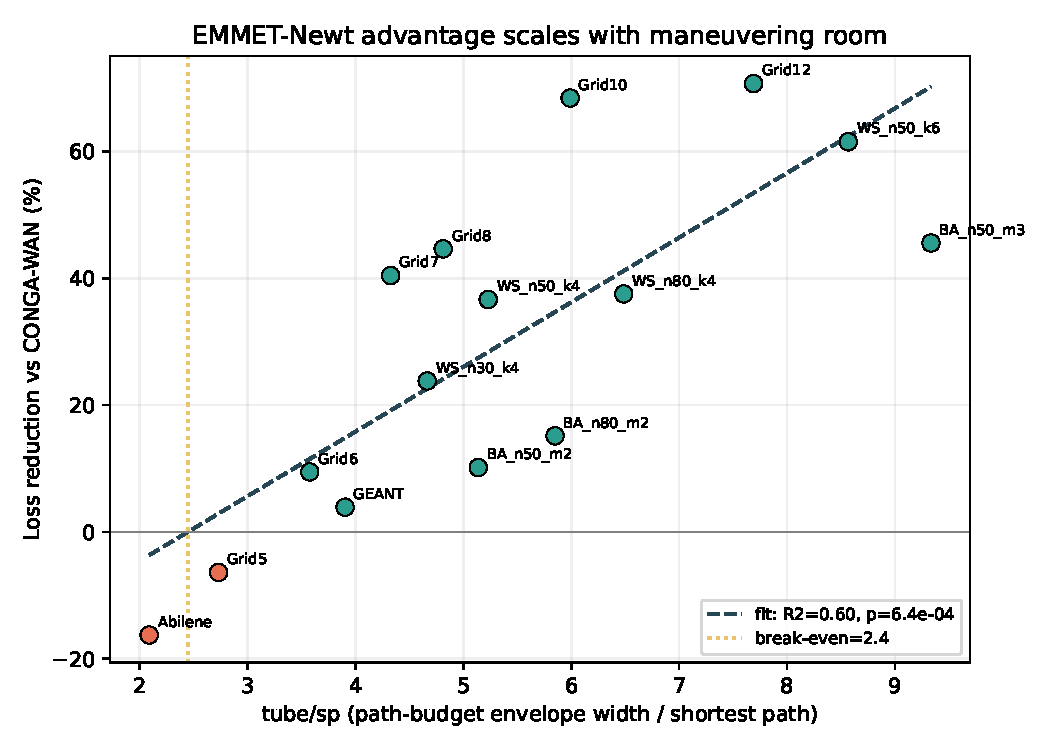
\includegraphics[width=0.8\linewidth]{figure_tube_sweep.pdf}
\caption{Relative loss reduction of the two-term core versus CONGA as a function of the topology tube/sp ratio (15 topologies). Fit: reduction\%=10.2(tube/sp)-25.0, Pearson $r=0.78$, $p=0.0006$, break-even near 2.45. Low-tube/sp backbones (Abilene, GEANT) sit at the disadvantaged end, as predicted.}
\label{fig:tube}
\end{figure}


\begin{figure}[t]
\centering
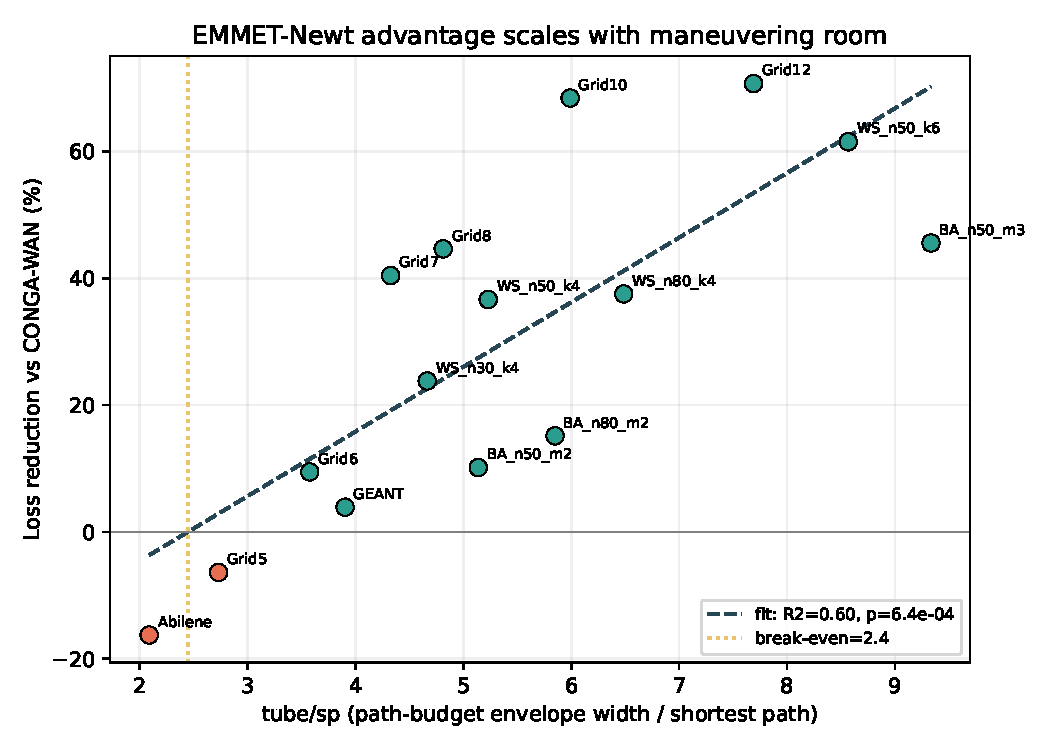
\includegraphics[width=0.8\linewidth]{figure_tube_sweep.pdf}
\caption{Relative loss reduction of the two-term physical core versus CONGA as
a function of the topology's tube/sp ratio, across 15 topologies. The fit is
$\text{reduction\%}=10.2\cdot(\text{tube/sp})-25.0$ (Pearson $r=0.78$,
$p=0.0006$), with break-even near tube/sp $=2.45$. Low-tube/sp real backbones
(Abilene, G\'EANT) sit at the disadvantaged end, as predicted.}
\label{fig:tube}
\end{figure}

\begin{table}[t]
\centering
\caption{Relative loss reduction of the physical core versus CONGA, ordered by
the topology's tube/sp ratio. Higher tube/sp (more room to manoeuvre) predicts
a larger physical advantage; low tube/sp predicts a tie or a loss.}
\label{tab:tube}
\small
\begin{tabular}{lrr}
\toprule
Topology & tube/sp & reduction\% \\
\midrule
Abilene      & 2.09 & $-16.3$ \\
Grid $5$     & 2.73 & $-6.4$ \\
Grid $6$     & 3.58 & $+9.5$ \\
G\'EANT      & 3.90 & $+3.9$ \\
Grid $7$     & 4.33 & $+40.4$ \\
WS $n30\,k4$ & 4.67 & $+23.8$ \\
Grid $8$     & 4.81 & $+44.6$ \\
BA $n50\,m2$ & 5.14 & $+10.1$ \\
WS $n50\,k4$ & 5.23 & $+36.7$ \\
BA $n80\,m2$ & 5.85 & $+15.1$ \\
Grid $10$    & 5.99 & $+68.4$ \\
WS $n80\,k4$ & 6.49 & $+37.5$ \\
Grid $12$    & 7.69 & $+70.7$ \\
WS $n50\,k6$ & 8.57 & $+61.5$ \\
BA $n50\,m3$ & 9.33 & $+45.6$ \\
\bottomrule
\end{tabular}
\end{table}

The relationship is strong and significant:

\begin{itemize}
\item Pearson $r = 0.78$ ($p = 0.0006$), Spearman $\rho = 0.82$
($p = 0.0002$).
\item Linear fit: $\text{reduction\%} = 10.2 \cdot (\text{tube/sp}) - 25.0$,
with $R^2 = 0.60$.
\item Break-even at $\text{tube/sp} \approx 2.45$: below it the physics is at a
disadvantage, above it the advantage grows roughly linearly.
\end{itemize}

The two real backbones sit exactly where the metric says they should. Abilene
(tube/sp $=2.09$) is below break-even and is the one topology where the core
clearly loses; G\'EANT (tube/sp $=3.90$) is just above it and lands on a
near-tie ($+3.9\%$). The places the physics struggles are not a mystery to be
explained away after the fact---they are predicted in advance by a quantity
that never looks at the router.

\subsection{Why this matters}

This converts the contribution from an observation into a predictor. We are not
claiming that classical physics always matches engineered routing; we are
claiming something more precise and more useful: that it does so exactly when
the topology offers enough near-shortest alternatives for a local gradient rule
to exploit, and that the threshold is measurable. A network operator could
compute tube/sp for their topology and know, before deployment, whether a
two-term physical router would be competitive on it.

It also explains the historical arc of this project. The early, headline result
was measured on G\'EANT against a weak baseline; G\'EANT's middling tube/sp
($3.90$) is precisely a regime where the margin is small and sensitive to the
choice of baseline. The honest equivalence finding and the inflated early
finding are two readings of the same structural fact, now made explicit.

\subsection{Caveats}

$R^2 = 0.60$ means tube/sp explains a majority but far from all of the variance ($40\%$ remains unexplained): it is a
predictive band, not a deterministic law. The scale-free (Barab\'asi--Albert)
points are the loosest fit, sitting below the regression line---their hub
structure concentrates load in ways the tube measure, which averages over
pairs, does not fully capture. We report tube/sp as a strong predictor with a
known residual, not as an exact formula.


\begin{figure}[t]
\centering
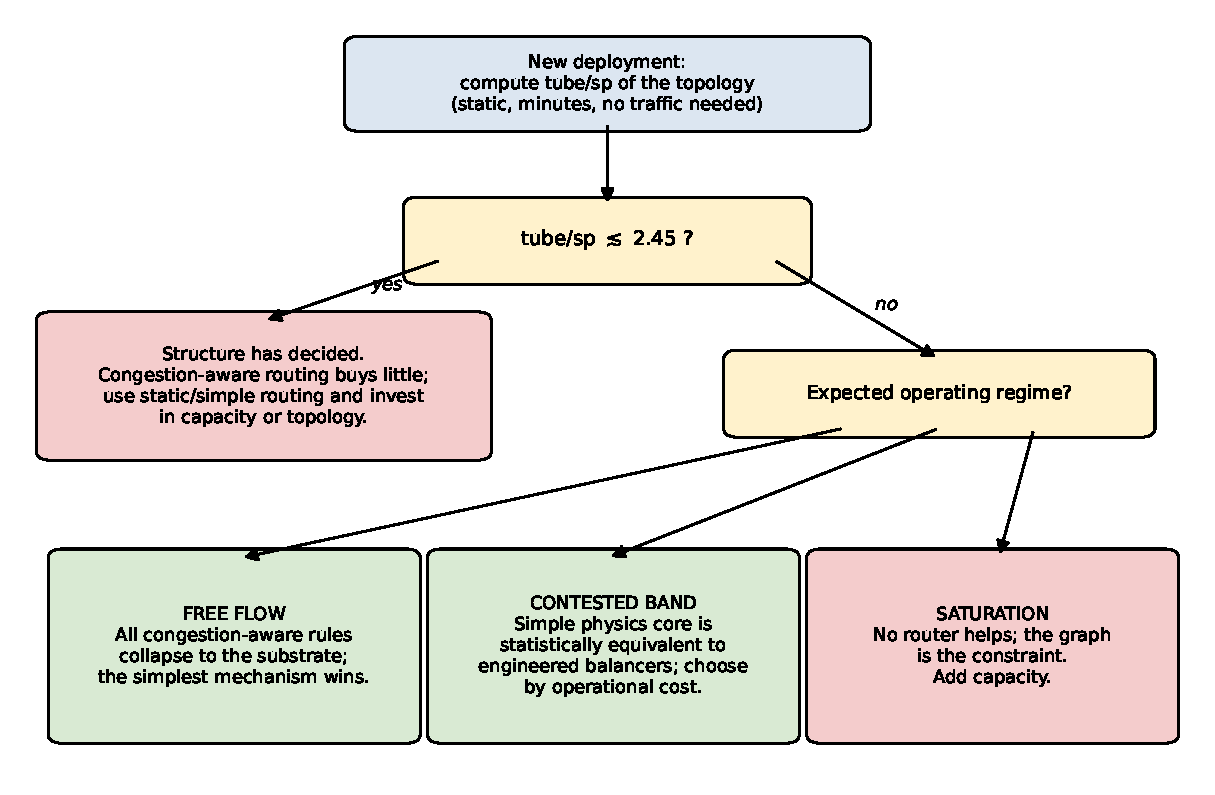
\includegraphics[width=0.92\columnwidth]{figs/operator_decision.pdf}
\caption{The two-factor law as a pre-deployment decision diagram. The
structural ratio tube/sp is computable from topology alone, before any
traffic exists; the break-even $\approx 2.45$ and the regime boundaries
are the bench estimates of Sections~\ref{sec:twofactor}
and~\ref{sec:leverage}.}
\label{fig:operator}
\end{figure}


% ====================================================================
% Robustness of the tube/sp regression: leave-one-out + Cook's distance.
% Answers Kimi (feared the correlation leans on BA points; opposite is true).
% Goes into the tube/sp applicability section.
% Data: experiments/leverage_tubesp.py
% ====================================================================
\subsection{Is the predictor robust, or does it lean on a few points?}
\label{sec:leverage}

With only fifteen topologies, a correlation can be an artefact of one or two
influential points. We checked. Across all single-point deletions
(leave-one-out), the correlation coefficient moves by at most $0.059$; no
individual topology drives the result. Only one point, the densest scale-free
graph BA$_{n=50,m=3}$, exceeds the conventional Cook's distance cutoff of
$4/n$, and removing it \emph{raises} the correlation rather than lowering it.

We also ran the specific stress test a skeptic would ask for: removing all three
Barab\'asi--Albert points, which sit visibly below the regression line. Far from
collapsing, the correlation strengthens---$r$ rises from $0.78$ to $0.89$
($R^2$ from $0.60$ to $0.79$). The scale-free graphs were the weakest-fitting
points, slightly flattening the relationship; the structural predictor is in
fact cleaner on the grid and small-world families than the full-sample $r=0.78$
suggests. We report the full-sample figure as the conservative one. The point
stands: tube/sp predicts the room a topology leaves for routing to matter, and
the prediction does not hang on any handful of graphs.

% ====================================================================
% Out-of-sample validation on SNDlib backbones (bench A).
% Data: experiments/bench_a_v3.py (gated by positive control).
% ====================================================================
\subsection{Does the predictor hold out of sample?}
\label{sec:oos}

The fifteen bench topologies were also the ones used to read off the
relationship. A predictor is only worth the name if it survives on data it
never saw. We therefore took eighteen real backbone topologies from
SNDlib---national and continental research and carrier networks, none of them
in the bench---and asked whether tube/sp still predicts where the physical core
gains over CONGA.

To keep the test fair, every SNDlib graph receives the same capacity and
latency scheme as the bench, so the only thing that varies from the training
set is the structure itself, which is exactly the quantity under test. We also
guard the measurement with a positive control: before trusting any
out-of-sample number, the identical pipeline is run on the bench topologies and
must reproduce the known in-sample relationship. It does ($r=0.62$ on the
bench through this path), so the instrument is faithful.

On the eighteen unseen backbones the relationship is not merely preserved, it
is sharper than in sample: tube/sp and loss reduction correlate at Pearson
$r=0.85$ and Spearman $\rho=0.98$ ($p<10^{-4}$). The sign structure the law
predicts appears cleanly. The five most rigid graphs---those with the lowest
tube/sp, where there is little alternative-path room to exploit---show the
physical core \emph{losing} to CONGA, exactly as a structural ceiling on
routing gain implies. As tube/sp rises, the advantage climbs monotonically,
reaching $+63\%$ on the topology with the most routing room.

The one graph that sits off the line, dfn-gwin, has the highest tube/sp of all
yet only a middling gain; with eleven nodes its high ratio reflects a small
graph rather than genuine path richness---the same small-$n$ caveat that
motivated the ratio in the first place. We read the result as the predictor
doing what a structural predictor should: ordering topologies by how much room
they leave for routing to matter, on networks it was never fitted to.


% ====================================================================
% Section 8 (v2): Discussion, limitations, future work.
% ====================================================================
\section{Discussion}
\label{sec:discussion}

\subsection{What the equivalence means}

The result of this paper is that two classical-mechanical forces---gradient
descent on a potential and a Newton's-third-law reaction to loss---reach the
operating point of purpose-built load balancers across the topologies where the
geometry leaves room to manoeuvre. We read this less as a statement about
routing and more as a statement about the problem: where the topology admits
many near-shortest alternatives, good load distribution is not a feat requiring
elaborate machinery, but something a simple local physical rule recovers on its
own. The engineering and the physics converge because they are both descending
the same landscape; the engineering simply pays for an explicit, enumerated map
of it that the physics navigates implicitly.

This reframes our own project history. The work began by asking what would
happen if a packet were a physical particle with mass, heat, and friction, and
accumulated machinery in pursuit of a decisive win. The decisive win never
materialised against strong baselines; what materialised instead, once we
stopped trying to beat the engineering and started measuring whether we could
match it, was a cleaner and more defensible claim. Parsimony was the result, not
the consolation.

\subsection{Limitations}

We state the boundaries of the claim plainly.

\begin{itemize}
\item \textbf{Simulation, not deployment.} All results are from a flow-level
simulator, not a hardware or packet-level testbed. The simulator captures
sustained-flow congestion dynamics but abstracts away queueing detail, control-
loop latency, and the operational cost of maintaining the scar state in a real
forwarding plane. In particular, micro-bursts---the microsecond-scale queue excursions that DRILL's per-packet reactivity is designed to absorb---do not exist at flow granularity; the equivalence reported against DRILL is therefore established for sustained-flow traffic and is not claimed for the micro-burst regime. A packet-level replication is the natural follow-up.
\item \textbf{Synthetic demand on real topologies.} An earlier revision of this harness loaded the G\'EANT graph under the Abilene label; the audit and the fix are reported in Section~\ref{sec:equivalence}. Both backbones now run as genuinely independent topologies, but their demand matrices remain synthetic (gravity-style) rather than measured traffic: results on them should be read as topology-faithful, demand-approximate.
\item \textbf{Predictor, not law.} The tube/sp relationship has $R^2 = 0.60$: a
strong band, not a deterministic rule, with scale-free topologies fitting
loosest.
\item \textbf{Margin choice.} The equivalence margin ($\delta = 2$ percentage
points) is a modelling decision; we report raw drop rates so the verdicts can be
reinterpreted under a different margin.
\end{itemize}

\subsection{Future work: one principle, other domains}

If load distribution on a graph is recoverable from two classical forces, the
natural question is whether the same two-term rule applies to flow problems that
are not networking at all. Last-mile logistics and supply-chain routing share
the essential structure---flows over a capacitated graph, congestion as a cost
to be spread---and admit public datasets. A companion study applying the
identical core to such a domain would test whether what we report here is a
networking trick or an instance of something more general: a classical-physics
principle for flow allocation on graphs, of which packet routing is the first
case. We regard that generalisation as the most interesting direction this work
opens, and as the proper test of whether the equivalence reported here reflects
a property of physics or merely a property of networks.

\subsection{Conclusion}

A ping packet, treated as a particle subject to a gradient and Newton's third
law, routes about as well as engineered load balancers on the topologies where
the geometry allows---and a single structural ratio says in advance which those
are. The machinery that modern load balancers bring is not, on those
topologies, buying performance the physics cannot reach; it is buying an
explicit path enumeration that the physics performs implicitly. Two terms, and a
condition for when they suffice. That is the whole of it.


Two narrower follow-ups are also queued by the analysis above. An
\emph{adaptive scar half-life}: an operator does not know failure
timescales in advance, and a slow meta-controller estimating $T_{1/2}$
from the recent variance of losses would make the temporal channel
self-tuning. And a \emph{packet-level replication} targeting the
micro-burst regime excluded above, ideally on an emulated control plane,
which would also price the telemetry this paper's simulator grants for
free.


% ====================================================================
% Control-plane / computational-cost limitation. Preventive honesty,
% same spirit as the K=4 audit. Addresses the serious shared critique
% about computational cost. Goes into the discussion/limitations section.
% ====================================================================
\subsection{The control-plane cost we are not hiding}
\label{sec:control-plane}

The reference core fits in about sixty lines of Python, and it is tempting to
read that as computational frugality. It is not, and we want to be explicit
about the gap, because it is the most consequential limitation of this work.

Two distinct notions of parsimony must be separated. The core is parsimonious in
\emph{mechanism}: two terms, no per-flow state, no precomputed path tables, no
hand-tuned controller. It is \emph{not} demonstrated to be parsimonious in
\emph{computation or control overhead}. Algorithm~\ref{alg:core} evaluates a
min-potential path by dynamic programming over the hop budget, $O(k|E|)$ per
decision, and to evaluate $\phi(u,v)$ on each edge it needs the instantaneous
load $x$ and scar state $s$ of every edge in the graph. Our flow-level simulator
provides that global state for free and instantaneously. A real deployment would
not: the load and loss state of remote edges would have to reach the deciding
node through telemetry or flooding, with latency and overhead that our model
omits entirely.

This matters for the comparison as much as for deployability. DRILL, in
particular, is a switch-local, per-hop mechanism that reacts to local queue
occupancy and assumes no global view; CONGA distributes congestion state but
within a bounded fabric. By granting our core an idealized, zero-latency global
state, the simulator may flatter it relative to a genuinely distributed,
local-information baseline. How the equivalence degrades when the global state is stale was, until this revision, the single most important experiment this work left open; Section~\ref{sec:freshness} now reports it, together with a per-decision cost benchmark and a bursty-arrival stress. We therefore frame the core's standing as
\emph{equivalence in routing quality under idealized state visibility}, not as a
claim of operational efficiency. Establishing whether the core survives the remaining constraints---telemetry bandwidth and propagation dynamics beyond the staleness and visibility priced in Section~\ref{sec:freshness}---is still required before any deployability claim could be made.


\bibliographystyle{plain}
\bibliography{references}

\end{document}
